\documentclass[long, final]{jobim}
% Available options are:
% - showframe
% - draft
% - final [default]

\usepackage[utf8]{inputenc}
\usepackage[T1]{fontenc}
\usepackage{siunitx}
\usepackage{amsmath, amssymb}
\usepackage{csquotes}
\usepackage{mathtools} % to get text over symbol
\usepackage{multicol} % for mini-pages
\usepackage{enumitem} % customised lists
\usepackage[square, sort&compress, numbers]{natbib}
\usepackage{listings}
\usepackage{tensor}


% define R packages and use R code
\newcommand{\CRANpkg}[1]{\href{https://CRAN.R-project.org/package=#1}{\textbf{#1}}}



% define the generalised tensor product
\newcommand{\cdotT}[1]{\stackrel{\mathclap{
#1}}{\quad \cdot \quad}}
% examples
% $$
% A \cdotT{i_1=i_3} B \quad
% A \quad \stackrel{\mathclap{i_1=i_3}}{\cdot} \quad B
% $$
% \stackrel{\mathclap{\text{def}}}{=}

\usepackage[svgnames]{xcolor} % with the set of colors to be used
\lstset{language=R,                                     % set programming language
    basicstyle=\small\ttfamily,                         % basic font style
    stringstyle=\color{DarkGreen},
    otherkeywords={0,1,2,3,4,5,6,7,8,9},
    keywordstyle=\color{Blue},                          % keyword style
    commentstyle=\ttfamily \color{DarkGreen},           % comment style
    backgroundcolor=\color{AliceBlue},                  % background colour
    numbers=left,                                       % display line numbers on the left side
    numberstyle=\ttfamily\color{Gray}\footnotesize,     % line numbers
}

% maths operators
% Optimisation
\DeclareMathOperator*{\argmax}{arg\,max}
\DeclareMathOperator*{\argmin}{arg\,min}

% matrix operators
\DeclareMathOperator*{\Tr}{Tr}
\DeclareMathOperator*{\DET}{Det}
\DeclareMathOperator*{\diag}{Diag}

% Probability Operators
\DeclareMathOperator*{\prob}{\mathbb{P}}
\DeclareMathOperator*{\esp}{\mathbb{E}}
\DeclareMathOperator*{\var}{\mathbb{V}\text{ar}}
\DeclareMathOperator*{\cov}{\mathbb{C}\text{ov}}
\newcommand \PP [1]{\prob\left({#1}\right)}
\newcommand \EE [1]{\esp\left[{#1}\right]}
\newcommand \VV [1]{\var\left[{#1}\right]}
\newcommand \CC [1]{\cov\left[{#1}\right]}

% Sets
\newcommand \NN {\mathbb{N}}
\newcommand \ZZ {\mathbb{Z}}
\newcommand \QQ {\mathbb{Q}}
\newcommand \RR {\mathbb{R}}



\pagestyle{empty}
\addtolength{\parskip}{0.4\baselineskip}

%% Title of the paper (required)
%\title{Template for \jobim2023 Proceedings [Titre/Title]}
\title{DeCovarT: Robust deconvolution of cell mixture in transcriptomic samples by leveraging cross-talk between genes}

%% List of authors (separated by the macro \and).
%% Authors can be followed by \inst{<n>} macro.
%% The <n> parameter of the \inst macro should correspond to the <n>th institution
%% (see macro \institute below).
\author{Bastien \textsc{CHASSAGNOL}\inst{1, 2}  \and Yufei \textsc{Luo}\inst{1} \and Gregory \textsc{Nuel}\inst{2} \and Etienne \textsc{Becht}\inst{1}}

%% List of institutions (separated by the macro \and).
\institute{
 Les Laboratoires Servier, 50 Rue Carnot, 92150, Suresnes, France
 \and
 LPSM (Laboratoire de Probabilités, Statistiques et Modélisation),  4 place Jussieu, 75005, Paris, France
}

% email of the corresponding author
\corresponding{bastien.chassagnol@upmc.fr}

% \papername{Meert \textit{et al.} (2016) Unknown species discovered by metagenomics
%   of frikandels. \textit{Annals of Improbable Research}. \url{http://dx.doi.org/11.0110/0111/111-1110-0001}}

%% Abstract of the paper (required).
\abstract{%
 \textbf{Motivation:} Transcriptomic analyses have increasingly contributed to our understanding of the biological processes involved in the pathophysiology of complex diseases. However, conventional bulk analyses ignore the intrinsic complexity of biological samples, by averaging measurements across multiple distinct cell populations. Furthermore, single-cell sequencing is a destructive and burdensome process, requiring in particular the dissociation of tissues into individual cells.
To leverage historical RNAseq analysis or to study fibrous tissues, computational deconvolution methods are still required to unravel the heterogeneous composition of biological samples. However, the performance of these algorithms is hampered by their strong assumption that gene expression is independent of each other, which prevents them from disentangling closely related cell types.

\textbf{Results:} We developed a new deconvolution algorithm, DeCovarT, that accounts for the network structure of each purified transcriptomic cell profile. Briefly, we hypothesise that transcriptomic interactions could be modelled by a multivariate Gaussian distribution, parametrised by a sparse precision matrix whose non null inputs represent direct connections between the genes. Finally, we assume that each mixture profile could be reconstructed by a linear combination of each purified transcriptomic cell profile, characterised by their \textit{plugged-in} covariance estimated beforehand by the gLasso algorithm. The cell ratios are then simply the weighted parameters, inferred in our paper by a constrained and reparametrised version of the Levenberg–Marquardt algorithm, which globally optimises the resulting convolution of Gaussian distributions.

We highlight that not only the distance between centroids (namely the mean differences between gene expression), but also the structure of the transcriptomic crosstalk, were relevant for selecting the minimal subset of genes to unambiguously characterise each cell population. Using this integrated approach, we obtained a mean correlation of 0.998 (\qty{95}{\percent} CI 0.995–0.999) from the RNA sequencing data of 35 whole blood samples over … cell populations, comparable to other standard deconvolution methods, such as deconRNAseq, CIBERSORT or MuSiC, while taking advantage of additional gene sets that were overlooked by other methods. We were also able to distinguish closely related cell populations with similar mean expression profiles but divergent transcriptomic structure.

}

%% List of keywords of the paper (required).
\keywords{\texttt{cellular deconvolution}, \texttt{gLasso}, \texttt{generative model}, \texttt{bulk RNA Sequencing}, \texttt{tumor micro environment}}

\begin{document}

\selectlanguage{english}

\maketitle

 \section{Introduction}
 \label{sec:introduction}

The analysis of the bulk transcriptome using high-throughput sequencing methods provided new insights on the mechanisms involved in the development of diseases. However, such methods obliterate the intrinsic heterogeneous nature of biological samples and thus reveal generally worthless to identify the causal sources of the variability observed between individuals.

Indeed, on par with the technical noise or the phenotypical environment, the cell composition plays a crucial role on the evolution of disease conditions. For instance, the tumoral micro environment encompasses a large variety of cell populations, whose interactions will directly impact the tumoral growth, cancer progression and henceforth the patient outcome). Furthermore, the expression profiles of a given cell population can even significantly differ within the same individual, driven by signalling pathways which induce \textit{cell motility} and \textit{cell differentiation} \cite{shoemaker_etal12}.

Not accounting for changes of the cell composition as one of the biological drivers as a confounding signal in downstream analyses, particularly in differential analysis, is likely to result in a loss of \textit{specificity} (genes wrongly identified as differentially expressed, while they only reflect an increase of the cell population naturally producing them) and \textit{sensibility} (genes expressed by minor cell populations are amenable to be masked by the expression and high-variability of dominant cell populations), which in turn prevents from identifying the true causal drivers of the change of gene dysregulation \footnote{\cite{whitney_etal03} shows that most of the inter-variability of gene expression within healthy patients was brought by variations of the neutrophils population, the major population of blood samples, making up for up to \qty{70}{\percent} of the nuclear-equipped cells}.

We can set apart two groups of technics for studying cell heterogeneity. Physical methods, such as immunohistochemistry and flow cytometry, can only take profit of a small subset of phenotypic markers to disentangle cell populations, making them burdensome, low-throughput and costly3. Single-cell sequencing (scRNASeq) is also a promising avenue, but disassociation of the tissues to isolate single cells prior to sequencing make them inconvenient to analyse deeply intertwined and fibrous tissues. Finally, a bench of computational methods were developed for estimating fractions of cell types in bulk admixtures, but they underperform for discriminating closely related cell types (e.g., naïve vs. memory B cells), due to their strong assumption of no interactions between genes. We thus introduce DeCovarT (Deconvolution using the Transcriptomic Covariance), a computational approach that we claim to provide unbiased and less noisy estimates, including ratios of closely related cell populations.


DeCovarT requires a larger compendium of purified RNASeq datasets to estimate for each purified cell population a vector of the averaged transcriptomic expressions and a precision matrix, assumed to be sparse.  With these inputs, we consider a generative model to rebuild the admixture of cell populations, assuming that the variability observed for each gene only stems from the stochastic nature of each cell population and its contribution to the global cell composition. To do so, we model the mixture by a convolution of multivariate Gaussian distributions, relaxing the assumption of Independence between observations (here, the individual expressions of transcripts), but keeping the assumption of Independence between covariates (here, the cell populations themselves), for identifiability and computational issues. Finally, the relative cell ratios were assigned the set of parameters that optimise the log-likelihood of the distribution, namely the MLE (maximum likelihood estimate).

We asserted the performance of our deconvolution algorithm by first characterising the network structure and the mean expression profile of the prevalent immune cell populations in blood vessels. ... genes enable to distinguish ... human hematopoietic cell phenotype, including ...

We then benchmarked DeCovarT on idealised mixtures with well-defined composition, and compared it with six GEP deconvolution methods —linear least squares regression (LLSR)4, quadratic programming (QP)5, PERT6, robust linear regression (RLR), MMAD7 and DSA8 (Supplementary Table 3). We next investigated more specifically the DeCovarT’s ability to disentangle highly correlated cell types, for which it was nearly unfeasible to identify any DEG (differentially expressed gene). Eventually, we asserted its performance on real datasets, for which FACS measurements of cell types were paired with bulk RNASeq analyses \textcolor{red}{page 4 and 5 of Cibersort}, we observed significant improvement over  other expression-based methods. Specially, some cell types, likely owing to multicollinearity, were more proned to \enquote{drop out} and system underestimation.

\section{Material and Methods}
\label{sec:methods}

\subsection{RNA sequencing datasets and preprocessing}
\label{subsec:preprocessing}

\subsection{Optimisation of the signature matrix}
\label{subsec:signature-matrix}

\subsubsection{Discard background noise}
\label{subsubsec:background-noise}

\subsubsection{Estimate a sparse transcriptomic network}
\label{subsubsec:gLasso}

\subsubsection{Multi-objective optimisation criterion for gene feature selection}
\label{subsubsec:genetic-algorithm}

\subsection{Overview of DeCovarT}
\label{subsec:DeCovarT}

Similar to most of transcriptomic deconvolution models, we assume that the total mRNA of a sample can be reconstructed by summing the individual contributions of each cell population weighted by its proportion. Formally, let \(\boldsymbol{X}=(x_{gj}) \in \mathbb{R}_+^{G\times J}\) the signature matrix storing the purified transcriptomic profiles of $J$ cell populations and \(\boldsymbol{p}=(p_{ji})\in [0, 1]^{J \times N}\) the unknown relative proportions of cell populations in $N$ samples, then the linear relation linking the bulk global expression $(\boldsymbol{y}=(y_{gi}) \in \mathbb{R}_+^{G\times N}$ to the individual cellular expression profiles is matricially described by: \equationname~\ref{eq:deconvolution-problem}:
\begin{equation}
\label{eq:deconvolution-problem}
\boldsymbol{y}=\boldsymbol{X} \times \boldsymbol{p}
\end{equation}


The positive constraints on the transcriptomic expressions proceed from the ability of NGS to retrieve RNA counts, and like most deconvolution methods, we are interested in retrieving the relative cell population ratios, assuming no additional undescribed cell subtype in the mixture (\equationname ~\ref{eq:positive-ratios}):
\begin{equation}
\label{eq:positive-ratios}
\begin{cases}
\sum_{j=1}^J p_{j}=1\\
\forall j \in \widetilde{J} \quad p_j\ge 0
\end{cases}
\end{equation}


Without noise or confusing variable, the solution to \equationname ~\ref{eq:deconvolution-problem} is unique (\textit{determined}) if the number of genes is at least equal to the number of cell types and no purified cellular expression profile can be rewritten as a linear combination of the other cell populations \footnote{Alternatively, non multicollinearity is guaranteed if the reference matrix \(\boldsymbol{X}\) is invertible and of full rank \(J\)}. When the number of genes exceeds the population cardinal, and in presence of confusing noise, the problem gets \textit{overdetermined}, with several conflicting solutions.

Most deconvolution methods handle the issue using \textit{linear regression techniques}: for a given sample, they proceed by minimising the Euclidean distance between observed values, noted \(\boldsymbol{y_i}\), and the predicted values, \(\boldsymbol{\hat{y_i}} \), enforcing the linear constraint defined in \equationname ~\ref{eq:deconvolution-problem} of the set of co-variables. The method, called OLS \textit{ordinary least squares}, is explicitly stated in \equationname ~\ref{eq:OLS}, with its matricial solution in \equationname ~\ref{eq:OLS-estimate}:

\begin{equation}
 \label{eq:OLS}
 \boldsymbol{\hat{p}}_{i}^{\text{OLS}} \equiv \argmin_{\boldsymbol{p}_i} ||\hat{\boldsymbol{y}_i} - \boldsymbol{y}_i||^2 = \argmin_{\boldsymbol{p}_i}  ||\boldsymbol{X}\boldsymbol{p}_i - \boldsymbol{y}_i||^2 = \sum_{g=1}^G \left( y_{gi} - \sum_{j=1}^J  x_{gj} p_{ji}\right)
\end{equation}

\begin{equation}
    \label{eq:OLS-estimate}
    \boldsymbol{\hat{p}}_{i}^{\text{OLS}} = (\boldsymbol{X}^\top\boldsymbol{X})^{-1}\boldsymbol{X}^\top \boldsymbol{y}_i
\end{equation}


An alternative method consists of deriving a \textit{generative model} that models the variability of the measured observations by drawing them from parametric probability density functions. The set of parameters, $\boldsymbol{p}$, that described the best the observations, is termed the \textit{maximum likelihood estimate} (MLE). Formally, the MLE maximises the likelihood or the log-likelihood of observed data: $\ell(\boldsymbol{p}|\boldsymbol{y}, \boldsymbol{X}) \equiv \prob_{\boldsymbol{p}}(\boldsymbol{y}|\boldsymbol{X})$ for our conditional distribution and with $\boldsymbol{p}$ the ratios to maximise.

Under some strong assumptions, enumerated in \theoremname~\ref{th:MLE_estimate_univariate}, we can corroborate the OLS and the MLE estimate:

\begin{theorem}[\textbf{Gauss-Markov theorem}]
If the following assumptions hold,
\begin{enumerate}
    \item \textbf{Strong exogeneity}: The cell type-specific expression profiles are not random variables but rather fixed and constant observations, underlying implicitly that cell populations do no interact:
  \(\forall i \in \widetilde{J} \, ,  \forall j \in \widetilde{J}, \, i \neq j, \quad \CC{\boldsymbol{x_{.i}}, \boldsymbol{x_{.j}}}=0\).
  \item \textbf{Gaussian-Markov noise:} This hypothesis assumes an independent white Gaussian noise, of null mean and variance not depending on the gene (\textbf{homoscedasticity}), for the distribution of the error term. Formally, it is likewise to adding a Gaussian distributed error term, $y_{gi} = \sum_{j=1}^J  x_{gj}p_{ji} \, + \epsilon_{gi}, \, \epsilon_{gi} \sim \mathcal{N} \left(0, \sigma_{gi}^2\right)$, from which, directly injecting the exogeneity and homoscedasticity properties, we deduce the univariate Gaussian nature of the distribution of each transcript:

  $y_{gi} \sim \mathcal{N} \left(\sum_{j=1}^J  x_{gj}p_{ji}, \sigma_{i}^2 \right)$
  \item \textbf{Independence:} From the aforementioned Gaussian-Markov and exogeneity assumptions, we readily deduce that the gene expressions of the bulk measures are independent: \(\forall j \in \widetilde{G}, \forall k \in \widetilde{G}, j \neq k, \quad  \CC{y_{ji}, y_{ki}}=0\).
  \item \textbf{Completeness:} We assume no additional latent variable, such as a non-surveyed cell population, that would contribute to the variability of the bulk mixture.
\end{enumerate}
then, the corresponding MLE estimate is equal to the OLS estimate, solution of \equationname ~\ref{eq:OLS} that can be computed using the \textbf{Normal equations}. Additionally, the MLE is unique (only one global maximum of the log-likelihood function) and BLUE (best linear unbiased estimator), i.e. the unbiased estimator with the lowest variance.
\label{th:MLE_estimate_univariate}
\end{theorem}

However, in next section, we consider a new generative model where some of the Gaussian-Markov assumptions are thwarted. Additionally, since we suppose that the samples are uncorrelated, and that the cellular proportions are likely to largely differ, even from samples proceeding from the same individual, we drop the index $i$ for the consistency of the redaction, using the same reference matrix $\boldsymbol{X}$ and deconvolving independently all samples (this hypothesis is highly privileged in most deconvolution algorithms, since it eases parallel and high-throughput estimation of the cellular ratios).

% For convenience, we introduce the following shorthand:
% \begin{itemize}
%     \item \(\boldsymbol{x}_{j}\) is the expression of all genes included in the experiment for a given cell population in cell population \(j\)
%     \item \(\boldsymbol{y}_{i}\) is the bulk mixture in sample \(i\)
%     \item \(\boldsymbol{p_i}\) is the vector of relative cellular proportions in sample $i$
% \item \widetilde{J} is a shortcut to indicate the index set ranging from $j=1$ to J, and reciprocally for \widetilde{N} and \widetilde{G}
% \end{itemize}

\subsubsection{Deconvolution model}
\label{subsubsec:deconvolution-model}

The DeCovarT algorithm assumes that the $G$-dimensional vector $\boldsymbol{x}_{.j}$ characterising the transcriptomic expression of each cell population follows a multivariate Gaussian distribution: $\boldsymbol{x}_{.j} \sim \mathcal{N}_G(\boldsymbol{\mu}_{.j}, \boldsymbol{\boldsymbol{\Sigma}}_{j})$, explicitly given in \definitionname~\ref{def:multivariate-gaussian-distribution}.

\begin{definition}[\textbf{Multivariate Gaussian distribution}]
\label{def:multivariate-gaussian-distribution}
The multivariate Gaussian distribution of the random vector of size $G$ characterising each purified transcriptomic profile, $\boldsymbol{x}_j$, is:
\begin{equation*}
    \DET(2\pi\boldsymbol{\Sigma}_j)^{-\frac{1}{2}} \exp\left( -\frac{1}{2} (\boldsymbol{x}_j - \boldsymbol{\mu}_{.j}) \boldsymbol{\Sigma}_j^{-1} (\boldsymbol{x}_j - \boldsymbol{\mu}_{.j})^\top\right)
\end{equation*}
which is parametrised by:
\begin{itemize}
    \item \textbf{the mean vector:} $\boldsymbol{\mu}_{.j}$
    \item \textbf{the covariance matrix:} $\boldsymbol{\Sigma}_j$ is a $G\times G$ squared matrix, \textit{positive-definite} and \textit{full rank}, guaranteeing the identifiability and non-degeneracy of the distribution. $\boldsymbol{\Theta}_j \equiv \boldsymbol{\Sigma}_j^{-1}$ is the \textit{precision matrix}.
\end{itemize}
\end{definition}

By considering a multivariate point of view to describe the transcriptomic expression, we not only relax the exogeinity property required for \theoremname~\ref{th:MLE_estimate_univariate} (already considered in  DSection \cite{erkkila_etal10} and DeMixt \cite{wang_etal18}) but also the independence assumption between the observations. However, we keep the completeness assumption and the independent expression between the cell types, and we do not consider an additional technical error term, which would be specific of the bulk sample, and instead consider that all the variability stems from the stochastic nature of the purified expression profiles.




For the derivation of the log-likelihood, we first \textit{plug-in} the mean and covariance parameters $\zeta_j=\left(\boldsymbol{\mu}_{.j}, \boldsymbol{\Sigma}_j\right)$ for each purified cell population (\sectionname~\ref{subsec:signature-matrix}). Instead, $\boldsymbol{\zeta}$ stores the parameters of the resulting Gaussian multivariate conditional distribution, with $\boldsymbol{\mu} \in \mathcal{M}_{G \times J}$ the concatenated matrix of the mean expression of the $J$ purified cell populations and in $\boldsymbol{\Sigma} \mathcal{M}_{G \times G}$ the global covariance matrix of the conditional distribution $\boldsymbol{y}|(\boldsymbol{\zeta}, \boldsymbol{p})$.

The unknown parameters to infer are the cellular ratios $\boldsymbol{p}$. Then, considering the matricial relation \equationname ~\ref{eq:deconvolution-problem}, the conditional probability of the bulk admixture given the individual mean and covariance parameters of each purified cellular expression, $\boldsymbol{y}|\boldsymbol{\zeta}$, which is as a sum of random variables, the \textit{convolution product} of independent multivariate Gaussian variables, follows a multivariate Gaussian distribution. Indeed, the \textit{affine invariant} property of Gaussian distributions enable to derive an explicit form of the multivariate probability condition (\equationname~\ref{eq:conditional-multivariate-distribution}):
\begin{equation}
\label{eq:conditional-multivariate-distribution}
\boldsymbol{y}|(\boldsymbol{\zeta}, \boldsymbol{p}) \sim \mathcal{N}_G(\boldsymbol{\mu} \boldsymbol{p}, \boldsymbol{\Sigma}) \text{ with } \boldsymbol{\mu} = (\boldsymbol{\mu}_{.j})_{j \in \widetilde{J}}, \quad \boldsymbol {p}=(p_1, \ldots, p_J) \text{ and } \boldsymbol{\Sigma}=\sum_{j=1}^J p_{j}^2\boldsymbol{\Sigma}_{j}=
\boldsymbol{p}_{j_1}^2 \cdotT{j_1=j_2} \boldsymbol{\Sigma}\indices{_{ik}^{j_2}}
\end{equation}
with $\cdotT{j_1=i_3}$ the generalised tensor product (\definitionname~\ref{def:tensor-product}) between the vector of proportions, $\boldsymbol{p}$, along the third dimension $j_2$ of the three-dimensional array, $\boldsymbol{\Sigma}\indices{_{ik}^{j_2}}, \quad (i, k)\in \widetilde{G}^2, \, j_2 \in \widetilde{J}$, storing the respective covariance matrices of each purified cell population (we used the Einstein summation convention for that last equation, see \definitionname~\ref{def:einstein-summation}).
Finally, from \equationname~\ref{eq:conditional-multivariate-distribution}, we readily compute the log-likelihood:

\begin{equation}
\label{eq:loglikelihood-multivariate-gaussian}
\ell_{\boldsymbol{y} | \boldsymbol{\zeta}}(\boldsymbol{p})=C + \log\left(\DET \left(\sum_{j=1}^J p_{j}^2\boldsymbol{\Sigma}_{j}\right)^{-1}\right) - \frac{1}{2} (\boldsymbol{y} - \boldsymbol{p} \boldsymbol{\mu})^\top \left(\sum_{j=1}^J p_{j}^2\boldsymbol{\Sigma}_{j}\right)^{-1} (\boldsymbol{y} - \boldsymbol{p}\boldsymbol{\mu})
\end{equation} with $C=-\frac{G}{2}\log(2\pi)$ a constant.
\textcolor{red}{J'intègre les paramètres supposées connues de moyenne et de variance, la seule variable observée reste donc y, dépendante conditionellement de $\mu$ et $\Sigma$, je ne cherche donc pas à retrouver spécifiquement l'expression des cellules purifiées $\boldsymbol{X}$ pour mon échantillon. Pas trop sûr du choix de $\boldsymbol{mu}$, alors qu'ici, c'est la matrice des moyennes que je prends, et non un simple vecteur!!}

From the covariance matrix of the multivariate conditional distribution (\equationname~\ref{eq:conditional-multivariate-distribution}), provided some of the off-diagonal terms are not null, it is clear that the genes of the bulk expression are not anymore independent and that the individual variance of each gene depends on the predictors and on the parameters to estimate. As we detail comprehensively in Appendix, this will considerably hamper the estimation process.

% \begin{equation}
%     \ell_{\theta}(\boldsymbol{X}, \zeta)=C + \frac{1}{2} \log\left(\DET(\Theta)\right) - \frac{1}{2} \sum_{i=1}^N (\boldsymbol{x_i} - \mu)^\top \Theta (\boldsymbol{x_i} - \mu)
% \end{equation}

 % assuming that the biological and technical conditions underlying the phenotype of the sample in the purified cell distribution and the bulk mixture are similar

% \subsubsection{Derivation of confidence intervals}
% \label{subsubsec:confidence-intervals}

\subsubsection{Package implementation}
\label{subsubsec:implementation}

\subsubsection{Other GEP deconvolution methods}
\label{subsubsec:other-deconv-methods}

\section{Results}
\label{sec:results}

\subsection{Toy example on synthetic mixtures}
\label{subsec:sim-idealised}

To highlight the counter-intuitive effect of the multicollinearity between gene observations, we simply design a toy example with two genes and two cell proportions, the simplex constraint amounting to estimate a single free parameter. Interestingly, playing over the correlation between the two genes within a cell population and the distance between the two centroids (here, the two-dimensional mean expression vectors of each cell population), we illustrate with that really simple example that no direct relationship between the pairwise correlation between the transcripts and the overall quality estimation could be established. Rather, the level of overlap between two cell populations distributions was a much better proxy of the quality of the estimation: the less the two cell populations distributions overlie, the better the sensibility of the deconvolution. We also showcase that our method, accounting for the covariance structure, systematically performs better compared to a traditional least squares regression method that assumes independent observations.



\subsection{Performance on real biological use case}
\label{subsec:sim-real}



\section{Conclusion}
\label{sec:conclusion}
We introduced the first deconvolution algorithm that is based on a generative statistical model loosening the strong independence assumption of gene independence. Biologically, discarding this strong hypothesis makes sense, since sets of genes interplay together to perform intricate biological functions, in structures named pathways.
Statistically, benchmarking our results in whole blood samples with known FACS counts against DeconRNASeq \cite{gong_szustakowski13}, CIBERSORT \cite{newman_etal15}, MuSiC \cite{wang_etal19} and xCell \cite{aran_etal17} results in systematically better performance over a set of quality metrics. \textcolor{red}{Interestingly, the correlation for monocytes was the least accurate for all methods used, confirm this statement?, cf deconvSeq}. We are also able to leverage a new set of genes with close mean expression profiles but distinct co-expression patterns, which were traditionally discarded by other deconvolution methods. We hence believe that the higher flexibility of our deconvolution algorithm will make it relevant to increase the currently poor cell resolution of deconvolution methods, with an extended ability to discriminate highly correlated cell population.

\subsection{Limitations}
\label{subsec:limitations}

The sparse estimate of the precision matrix returned by the gLasso \cite{mazumder_hastie11} algorithm is generally shrunk, entailing in practice that the non null partial correlations are generally underestimated. \textit{Parameter shrinkage} is a common and well-documented issue of regularisation methods that penalise the complexity of the model. A way to circumvent this problem is to use the \textit{support} returned by the penalisation method to refine the estimation by a canonical maximum likelihood strategy that would integrate the topological constraints induced by the null inputs of the precision matrix (an item set to zero means no direct edge connecting the two transcripts). Unfortunately, except in really specific configurations in which the graph is \textit{chordal}, there is no single MLE solution that optimally capture the correlation structure of a set of observations.



The INDEED algorithm \cite{zuo_etal16} is tailored to select markers between two biological conditions only and not among several groups. While we worked around the problem by performing an one-vs-all strategy, such an approach is quite controversial, since this heuristic strategy does not account for the specificity of each cell profile, the remaining expression profiles being averaged, (discrimination of minor cell populations with lower depth sequencing are likely to be confused with such strategy), nor enable to identify collectively the minimal subset of genes able to discriminate any cell population. Additionally, the way the Indeed algorithm performs to combine the close transcriptomic neighbourhood and the mean expression within a single metric function is derogatory, since the units are not on the same scale.

Rather, a multi-objective and global optimisation approach seems an excellent alternative to manage the trade-off of neighbourhood and mean gene expression discrimination at the scale of a cell population. Finally, while exploring globally the space of gene subsets is generally infeasible due to the combinatorial explosion of possibilities ($2^G$ with $G$ the number of genes retained after background filtering), a genetic and evolutionary approach, likewise to the AutoGeneS algorithm \cite{aliee_theis21}), in which a population of candidate solutions are randomly modified (each solution is the bite wise or indicator function of a set of genes, a zero input representing a gene discarded) and iteratively optimised to finally return a collection of \enquote{Pareto-solutions} that represent on a two-dimensional plot the best trade off between the two metrics compared.


Finally, we could refine our generative model to integrate heterotypic interactions, namely accounting for modifications induced by a change of the environmental medium, like a the release of a signalling molecule or a dysregulation of the metabolic pathways induced by a genetic mutation, or a technical batch. A mixed linear-model could be used to account for known environmental and technical confusing factors. However, if no reference profile is available or the nature of the confusing variable is unknown, a better alternative would be to encompass any latent driver within a Bayesian framework, whose parameters of the prior distributions would be retrieved from the literature or FACS data on similar samples (for cell ratios) or from the plugged-in estimates of purified profiles extracted in similar environmental conditions (for the mean and covariance parameters). A Bayesian approach would also alleviate the difficulty of asserting the statistical relevance of the estimates, by directly returning from the simulation likelihood intervals.




\subsection{Perspectives}
\label{subsec:perspectives}

We assumed a multivariate Gaussian distribution to model our purified transcriptome. However, the original outputs returned by RNASeq approaches are discrete integer counts of transcripts that are better captured with Poisson or negative Binomial approaches. We circumvent this problem by using TPM normalisation, followed by a log2 transformation. However, doing so, we do not directly estimate the cellular RNASeq fractions, since we assume that the bulk mixture is a linear combination of the individual transcriptomic contributions of the raw counts, and not of the log2 normalised. While deconvSeq \cite{du_etal19} directly estimates the cell ratios on the original material, by modelling gene expressions by a negative binomial distribution, and Kassandra \cite{zaitsev_etal22} adds artificial Poisson environmental and technical noise to the inputs of its ensemble LightGbm regression approach, none of them accounts for the interaction between genes, the multivariate factor making the estimation hardly challenging.


While for the sake of simplicity, we consider since the beginning that the outputs returned by the deconvolution algorithms were directly the relative cell ratios, this is generally a misleading shortcut. What we compute indeed is rather the fraction of RNASeq produced by a given cell type, rather than the cell proportion itself \footnote{\cite{racle_etal17}highlights in supplementary Figure 1, panel A, the expected mRNA amount in common immune cell populations: while lymphocytes and NK cells, all highly associated in terms of cell lineage, display the same mRNA amount, around $0.4 \unit{pg}$, the quantity extracted from neutrophils is twice lower and 3 folds higher for monocytes.}. Indeed, the total amount extracted from a given cell is contingent on its size and on technical constraints that play on the efficiency of the RNA extraction. To yield the actual cellular ratio, we need to normalise the inferred cellular RNASeq fractions by dividing them by the expected total amount of RNA transcripts released within the cell population, as described in \equationname ~\ref{eq:normalisation-rna-extraction}:

\begin{equation}
    \hat{p^*_j} = K \frac{\hat{p_j}}{r_j}, \quad K= \frac{1}{\sum_{j=1}^J \frac{\hat{p_j}}{r_j}}
    \label{eq:normalisation-rna-extraction}
\end{equation}

with $r_j$ the average number of transcripts extracted per cell type and $K$ the normalisation constant asserting the unit simplex constraint. Previous studies handle this biased effect by either normalising back the inferred RNASeq ratios based on extraction experiences prior to the deconvolution (EPIC algorithm in \cite{racle_etal17} and QuantiSeq \cite{finotello_etal19}) or as an additional unknown parameter to infer (MMAD algorithm, in \cite{liebner_etal14}).

Finally, in complex tissues, such as the TME, there is always a part of the cell composition and expression that is undescribed, notably tumoral cells that mutated from germinal lines display over-expression or amplification of the expression of mutagen driver genes. Simply adding an intercept noise to account for these uncovered cell populations reveals generally inadequate, since this amounts to consider that the contribution of the unknown cell content is similar for any gene. Some deconvolution algorithms tailored this issue, by hypothesising that the unexplained cell transcriptomic profile is the scalar multiplication of one (ISOLATE algorithm \cite{quon_morris09}) or an additive linear combination of a subset of the ground cell populations (NNML\textsubscript{np} algorithm \cite{qiao_etal12}) \footnote{Considering that the unknown transcriptomic profile is a modified expression of one or more existing populations avoids that all the unexplained variability is captured by this unknown cell population}, by adding voluntarily some hyper-expression noise to avoid overfitting (the Kassandra algorithm uses an ensemble model refined on thousands of simulated mixtures, that reproduce high-leveraging confusing factors by adding globally a Poisson technical noise and for an \textit{ad-hoc} fraction of genes an uniform constant factor) or by preventing aberrant genes whose expressions were largely altered by somatic mutations from confounding the deconvolution results (robust linear regression or support vector regression, as in Cibersort algorithm, are two approaches that reveal efficient to discard aberrant gene expressions prior to the estimation stage).
 % \begin{figure}
 %   \begin{center}
 %     \setlength{\unitlength}{5mm}
 %     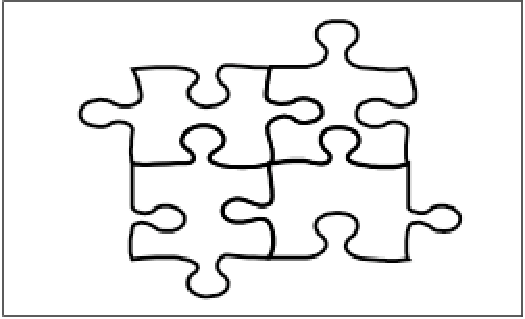
\includegraphics[height=4cm,width=6cm]{figs/fig1}
 %   \end{center}
 %   \caption{Old \jobim puzzle (end of the 20th century).}
 %   \label{fig:puzzle}
 % \end{figure}


\begin{acknowledgements}
  \label{sec:acknowledgements}
This study makes use of data generated by the Blueprint Consortium, whose proprietary use was granted for exploratory analysis to the company Les Laboratoires Servier. A full list of the investigators who contributed to the generation of the data is available from \url{www.blueprint-epigenome.eu}.

We would also like to thank the BBC team within my company who implemented the RNASeq pipeline that was used to preprocess and curate both purified and bulk RNA datasets. The code used for that section can be found on \href{https://github.com/orgs/servier-github/repositories}{Servier-Github}.

\end{acknowledgements}


 \bibliography{jobim_proceedings}


 \appendix

\section{Model}


\subsection{First and second-order derivation of the unconstrained DeCoVart log-likelihood function}
\label{subsubsec:uncontrained-optimisation}

To determine analytically the stationary points of a function, and notably its maximum, we need to determine the roots (the values for a which a function equals zero) of its gradient.  The gradient of a real-valued function, $l:\RR^J \to \RR$, is given by the vector indexing the partial derivatives evaluated at each of its coordinates.

However, before deriving the first and second-order derivatives of the log-likelihood function \equationname~\ref{eq:loglikelihood-multivariate-gaussian}, let's review basic requirements about linear algebra properties in \propertyname~\ref{pr:matrix-calculus-first-order} and matrix calculus at first order in \propertyname~\ref{pr:linear-algebra} that will considerably ease the calculations.

\begin{definition}[Positive-definite matrix]
\label{def:positive-definite}
A symmetric real matrix $\boldsymbol{A}$ of rank $G$ is said to be \textit{positive-definite} if $\boldsymbol{x}^\top \boldsymbol{A} \boldsymbol{x} > 0$ for all non-zero vectors $\boldsymbol{x}$ in $\mathbb{R}^G$.
\end{definition}

\begin{property}[Linear algebra properties]
\label{pr:linear-algebra}
First, we introduce below some properties associated to the determinant and trace operators. For a squared matrix $A$ of rank $G$ with defined inverse variance $A^{-1}$ and a constant $p$, the following properties hold:
\begin{multicols}{3}
\begin{enumerate}[label=\emph{\alph*})]
\item $\DET(p\boldsymbol{A})=p^G \DET (\boldsymbol{A})$
%\columnbreak
\item $\Tr\left(p \boldsymbol{A}\right)=p \Tr(\boldsymbol{A})$
%\columnbreak
\item $\DET(A^{-1})=\frac{1}{\DET(A)}$
\end{enumerate}
\end{multicols}

Then, we introduce some properties practical with the transpose operator, which switch the row and column indexes. Given two matrices $\boldsymbol{A}$ and $\boldsymbol{B}$, the following properties hold when computing their transpose:
\begin{multicols}{3}
\begin{enumerate}
    \item $(\boldsymbol{A}^\top)^\top=\boldsymbol{A}$
    \item $(\boldsymbol{A}\boldsymbol{B})^\top=\boldsymbol{B}^\top\boldsymbol{A}^\top$
    \item $\boldsymbol{A}^{{-1}^\top}=\boldsymbol{A}^{-1}$ with the additional constraint that $\boldsymbol{A}$ is a symmetric matrix.
\end{enumerate}
\end{multicols}


Another useful equality, given two vectors $\boldsymbol{x}$ and $\boldsymbol{y}$ in $\RR^G$ and $\boldsymbol{A}$ a symmetric matrix \footnote{if a matrix is symmetric, then by definition, $\boldsymbol{A}^\top=\boldsymbol{A}$} of rank $G$:
\begin{equation*}
    \boldsymbol{x}^\top \boldsymbol{A} \boldsymbol{y} = \boldsymbol{y}^\top \boldsymbol{A} \boldsymbol{x}
\end{equation*}
\end{property}

\begin{property}[\textbf{matrix calculus:} first order]
\label{pr:matrix-calculus-first-order}
Given two invertible, positive-definite matrices (see Definition in \ref{def:positive-definite}) $\boldsymbol{A}$ and $\boldsymbol{B}$, with respective inverses $\boldsymbol{A}^{-1}$ and $\boldsymbol{B}^{-1}$, $A=\boldsymbol{A}(p)$ and $B=\boldsymbol{B}(p)$ being functions of a scalar variable $p$, the following properties hold:
\begin{multicols}{3}
\begin{enumerate}[label=(\alph*)]
\item $\frac{\partial \DET(\boldsymbol{A})}{\partial p}=\DET(\boldsymbol{A}) \Tr \left(\boldsymbol{A}^{-1} \frac{\partial \boldsymbol{A}}{\partial p} \right)$
\item $\frac{\partial \boldsymbol{U}\boldsymbol{A}\boldsymbol{V}}{\partial p} = \boldsymbol{U} \frac{\partial\boldsymbol{A}}{\partial p} \boldsymbol{V}$
\item $\frac{\partial \boldsymbol{A}^{-1}}{\partial p} = -\boldsymbol{A}^{-1} \frac{\partial\boldsymbol{A}}{\partial p} \boldsymbol{A}^{-1}$
\end{enumerate}
\end{multicols}
From equation a), we can readily compute $\frac{\partial \log\left(\DET(\boldsymbol{A})\right)}{\partial p}= \Tr \left(\boldsymbol{A}^{-1} \frac{\partial \boldsymbol{A}}{\partial p} \right)$ using the chain rule applied to a logarithmic function. Additionally, the derivative is well-defined and continuous, since $\boldsymbol{A}$ is positive-definite, henceforth its determinant is strictly positive. Finally, using the linear algebras formulas stated in \propertyname~\ref{pr:linear-algebra}, we deduce directly that: $\frac{\partial \log\left(\DET(\boldsymbol{A}^{-1})\right)}{\partial p}=- \Tr \left(\boldsymbol{A}^{-1} \frac{\partial \boldsymbol{A}}{\partial p} \right)$.

Additionally, both the additive property:$\frac{\partial c_1 \boldsymbol{A} + c_2 \boldsymbol{B}}{\partial p}=c_1 \frac{\partial \boldsymbol{A}}{\partial p} + c_2 \frac{\partial \boldsymbol{B}}{\partial p}$, $c_1$ and $c_2$ constants, and the multiplicative property:$\frac{\partial \boldsymbol{A} \boldsymbol{B}}{\partial p}= \boldsymbol{A}\frac{\partial \boldsymbol{B}}{\partial p} + \boldsymbol{B} \frac{\partial \boldsymbol{A}}{\partial p}$ of the derivative operator hold similarly for matrices as for real valued functions.


Given three matrices $\boldsymbol{A}$, $\boldsymbol{C}$, $\boldsymbol{D}$ and two vectors of same size $\boldsymbol{b}$ and $\boldsymbol{e}$, none of them depending on variable $\boldsymbol{p}$, the partial derivative with respect to $\boldsymbol{p}$ of the quadratic form $(\boldsymbol{A} \boldsymbol{p} + \boldsymbol{b})^\top \boldsymbol{C} (\boldsymbol{D} \boldsymbol{p} + \boldsymbol{e})$ is:
\begin{equation*}
    \frac{\partial (\boldsymbol{A} \boldsymbol{p} + \boldsymbol{b})^\top \boldsymbol{C} (\boldsymbol{D} \boldsymbol{p} + \boldsymbol{e})}{\partial \boldsymbol{p}} = (\boldsymbol{D} \boldsymbol{p} + \boldsymbol{e})^\top \boldsymbol{C}^\top \boldsymbol{A} + (\boldsymbol{A} \boldsymbol{p} + \boldsymbol{b})^\top \boldsymbol{C} \boldsymbol{D}
\end{equation*}

Notably, using the properties associated to the transpose operator, enumerated in \propertyname~\ref{pr:linear-algebra}, setting $\boldsymbol{A} = \boldsymbol{D} = - \boldsymbol{x}$ as vectors in $\RR^G$,  $\boldsymbol{b} = \boldsymbol{e} = \boldsymbol{y}$ and $\boldsymbol{C}= \boldsymbol{Theta}$ a symmetric matrix, the derivative simplifies to :
\begin{equation*}
    \frac{\partial (\boldsymbol{y} - \boldsymbol{x} p)^\top \Theta (\boldsymbol{y} - \boldsymbol{x} p)}{\partial p} = -2  (\boldsymbol{y} - \boldsymbol{x} p)^\top \Theta \boldsymbol{x} = -2 \boldsymbol{x}^\top \Theta (\boldsymbol{y} - \boldsymbol{x} p)
\end{equation*}

\footnote{Some proofs about matrix calculus can be found in \cite{kaare12}.}
\end{property}


That is, for our specific function defined in \equationname~\ref{eq:loglikelihood-multivariate-gaussian}, the vector: $\nabla \ell: \RR^J \to \RR^J$ evaluated at point $\boldsymbol{p}=(p_1, \ldots, p_J)$ in $J-$dimensional space (\equationname~\ref{eq:gradient-general}), with $\boldsymbol{\zeta}$ the plug-in, supposed known mean and covariance parameters of each purified cell function:

\begin{equation}
\label{eq:gradient-general}
\nabla\ell_{\boldsymbol{y} | \boldsymbol{\zeta}} (\boldsymbol{p})=
\begin{bmatrix}
\frac{\partial \ell_{\boldsymbol{y} | \boldsymbol{\zeta}} (\boldsymbol{p})}{\partial p_1} \\
\vdots \\
\frac{\partial \ell_{\boldsymbol{y} | \boldsymbol{\zeta}}(\boldsymbol{p})}{\partial p_J}
\end{bmatrix}
\end{equation}


We derive only one component of the gradient vector since the computation is the same for any cell component ratio $p_j, j \in \widetilde{J}$ (\equationname~\ref{eq:derivative-log-likelihood-unconstrained}):

\begin{equation}
\label{eq:derivative-log-likelihood-unconstrained}
\begin{split}
\frac{\partial \ell_{\boldsymbol{y} | \boldsymbol{\zeta}}(\boldsymbol{p})}{\partial p_j} =&  \frac{\partial \log\left(\DET(\boldsymbol{\Theta})\right)}{\partial p_j} -\frac{1}{2} \left[\frac{\partial (\boldsymbol{y} - \boldsymbol{\mu} \boldsymbol{p})^\top}{\partial p_j}\boldsymbol{\Theta}(\boldsymbol{y} - \boldsymbol{\mu} \boldsymbol{p}) + (\boldsymbol{y} - \boldsymbol{\mu} \boldsymbol{p})^\top\frac{\partial\boldsymbol{\Theta}}{\partial p_j}(\boldsymbol{y} - \boldsymbol{\mu} \boldsymbol{p}) + (\boldsymbol{y} - \boldsymbol{\mu} \boldsymbol{p})^\top\boldsymbol{\Theta} \frac{\partial (\boldsymbol{y} - \boldsymbol{\mu} \boldsymbol{p})}{\partial p_j} \right]\\
=&-\Tr \left(\boldsymbol{\Theta} \frac{\partial \boldsymbol{\Sigma}}{\partial p_j} \right) - \frac{1}{2} \left[ - \boldsymbol{\mu}_{.j}^\top\boldsymbol{\Theta}(\boldsymbol{y} - \boldsymbol{\mu} \boldsymbol{p}) - (\boldsymbol{y} - \boldsymbol{\mu} \boldsymbol{p})^\top\Theta\frac{\partial \Sigma}{\partial p_j}\Theta(\boldsymbol{y} - \boldsymbol{\mu} \boldsymbol{p}) - (\boldsymbol{y} - \boldsymbol{\mu} \boldsymbol{p})^\top\boldsymbol{\Theta}  \boldsymbol{\mu}_{.j} \right] \\
=& \textcolor{red}{-2p_j \Tr \left(\boldsymbol{\Theta}\boldsymbol{\Sigma}_j\right)} +
\textcolor{blue}{(\boldsymbol{y} - \boldsymbol{\mu} \boldsymbol{p})^\top\boldsymbol{\Theta}  \boldsymbol{\mu}_{.j}} \, +
\textcolor{green}{p_j (\boldsymbol{y} - \boldsymbol{\mu} \boldsymbol{p})^\top\boldsymbol{\Theta} \Sigma_j \boldsymbol{\Theta} (\boldsymbol{y} - \boldsymbol{\mu} \boldsymbol{p})}
\end{split}
\end{equation}

However, the non-closeness form of this function makes it impossible to analytically retrieve its zeros (indeed, contrary to the standard least squares regression method, the parameter to optimise is intertwined with the variance, and determining the inverse of the resulting covariance matrix, while isolating $\boldsymbol{p}$ reveals unfeasible). Hopefully, as we detail in next section, numerical approximations can be used as proxy to retrieve the roots of a function, but they require the computation of the Hessian matrix. Additionally, the local properties of the Hessian matrix in the neighbourhood of the extremum give relevant insights on the nature of the extremum (for instance, it can discriminate topologically a maximum from a saddle point or a minimum).

To compute the Hessian matrix, we complete the matrix calculus properties detailed in \propertyname~\ref{pr:matrix-calculus-first-order} with the following second-order matrix calculus derivations (\propertyname~\ref{pr:matrix-calculus-second-order}):

\begin{property}[\textbf{matrix calculus:} second order]
\label{pr:matrix-calculus-second-order}
Given an invertible matrix $\boldsymbol{A}$ depending on a variable $p$, the following calculus formulas hold:
\begin{multicols}{2}
\begin{enumerate}[label=(\alph*)]
\item
$$ \frac{\partial^2 \boldsymbol{A}^{-1}}{\partial p_i \partial p_j} =  \boldsymbol{A}^{-1} \left( \frac{\partial \boldsymbol{A}}{\partial p_i } \boldsymbol{A}^{-1} \frac{\partial \boldsymbol{A}}{\partial p_j} - \frac{\partial^2 \boldsymbol{A}}{\partial p_i \partial p_j}  + \frac{\partial \boldsymbol{A}}{\partial p_j } \boldsymbol{A}^{-1} \frac{\partial \boldsymbol{A}}{\partial p_i}\right) \boldsymbol{A}^{-1}
$$
\item
$$
\frac{\partial \Tr \left(\boldsymbol{A}\right)}{\partial p_i} = \Tr  \left(\frac{\partial \boldsymbol{A}}{\partial p_i}\right)
$$


\end{enumerate}
\end{multicols}

Combining the derivative formula for the inverse of a matrix, given in \propertyname~\ref{pr:matrix-calculus-first-order} with the linearity of the trace operator and the chain rule formula yields in particular:
\begin{equation*}
    \frac{\partial^2 \log \left(\DET (\boldsymbol{A}^{-1})\right)}{\partial^2 p} = - \Tr  \left[\boldsymbol{A}^{-1}\frac{\partial^2 \boldsymbol{A}}{\partial^2 p_i}\right] +
\Tr  \left[\left(\boldsymbol{A}^{-1}\frac{\partial \boldsymbol{A}}{\partial p_i}\right)^2\right]
\end{equation*}


Finally, the generalised Leibniz product rule, given below , reproduced from \cite{mulla20}, is also valid for the derivation of any product of $m$ matrices depending on a scalar $p$ (we restrain the formula to the first order only):
\begin{equation*}
    \frac{\partial (\boldsymbol{A}_1 \ldots \boldsymbol{A}_m)}{\partial p} = \sum_{\boldsymbol{\pi}_m} \prod_{1\leq t \leq m}  \boldsymbol{A}_t^{k_t}
\end{equation*}
in which $\boldsymbol{\pi}_m = \{(k_1, \ldots k_m) \in \mathbb{N}_0^m \}: \sum_{i=1}^m k_t = 1$ ( $\boldsymbol{\pi}_m$ is the set of integer tuples of size $m$, whose total sum equals the order of derivation, here 1). At the first order, deriving a product of $m$ matrices is thus equivalent to sum all tuples of matricial products products, each deriving a different matrix.
\end{property}




The second derivative order, corresponding to the Hessian matrix of the log-likelihood (\equationname~\ref{eq:loglikelihood-multivariate-gaussian}) in $\mathcal{M}_{J \times J}$ is given by:
\begin{equation}
    \label{eq:hessian-log-likelihood-unconstrained}
\begin{aligned}
\mathbf{H}(\ell(\boldsymbol{p})) &= \mathbf{J}\left( \nabla \ell (\boldsymbol{p})\right)\\
\mathbf{H}_{i,i}& =
   \frac{\partial^2 \ell}{\partial^2 p_i} =
\textcolor{red}{-2\Tr \left(\boldsymbol{\Theta}\boldsymbol{\Sigma}_i\right) + 4p_i^2 \Tr \left(\left(\boldsymbol{\Theta}\boldsymbol{\Sigma}_i\right)^2\right)}
\textcolor{blue}{-2p_i(\boldsymbol{y} - \boldsymbol{\mu} \boldsymbol{p})^\top\boldsymbol{\Theta} \boldsymbol{\Sigma}_i \boldsymbol{\Theta} \boldsymbol{\mu_{.i}}\, - \boldsymbol{\mu}_{.i}^\top\boldsymbol{\Theta} \boldsymbol{\mu_{.i}}} \, - \\
& \textcolor{green}{2p_i (\boldsymbol{y} - \boldsymbol{\mu} \boldsymbol{p})^\top \boldsymbol{\Theta}\boldsymbol{\Sigma}_i\boldsymbol{\Theta}\boldsymbol{\mu}_{.i} \, -
(\boldsymbol{y} - \boldsymbol{\mu} \boldsymbol{p})^\top\boldsymbol{\Theta} \left(4p_i^2 \boldsymbol{\Sigma}_i \boldsymbol{\Theta} \boldsymbol{\Sigma}_i - \boldsymbol{\Sigma}_i \right)\boldsymbol{\Theta} (\boldsymbol{y} - \boldsymbol{\mu} \boldsymbol{p})}, \quad i \in \widetilde{J} \\
& = -2\Tr \left(\boldsymbol{\Theta}\boldsymbol{\Sigma}_i\right) + 4p_i^2 \Tr \left(\left(\boldsymbol{\Theta}\boldsymbol{\Sigma}_i\right)^2\right)
-4p_i(\boldsymbol{y} - \boldsymbol{\mu} \boldsymbol{p})^\top\boldsymbol{\Theta} \boldsymbol{\Sigma}_i \boldsymbol{\Theta} \boldsymbol{\mu_{.i}}\, - \boldsymbol{\mu}_{.i}^\top\boldsymbol{\Theta} \boldsymbol{\mu_{.i}} \, - \\
& (\boldsymbol{y} - \boldsymbol{\mu} \boldsymbol{p})^\top\boldsymbol{\Theta} \left(4p_i^2 \boldsymbol{\Sigma}_i \boldsymbol{\Theta} \boldsymbol{\Sigma}_i - \boldsymbol{\Sigma}_i \right)\boldsymbol{\Theta} (\boldsymbol{y} - \boldsymbol{\mu} \boldsymbol{p})\\
\mathbf{H}_{i,j} &=
   \frac{\partial^2 \ell}{\partial p_i \partial p_j} =
\textcolor{red}{4p_j p_i \Tr \left(\boldsymbol{\Theta}\boldsymbol{\Sigma}_j \boldsymbol{\Theta}\boldsymbol{\Sigma}_i \right)}
\textcolor{blue}{-2p_i(\boldsymbol{y} - \boldsymbol{\mu} \boldsymbol{p})^\top\boldsymbol{\Theta} \boldsymbol{\Sigma}_i \boldsymbol{\Theta} \boldsymbol{\mu_{.j}} - \boldsymbol{\mu}_{.i}^\top\boldsymbol{\Theta} \boldsymbol{\mu_{.j}}} \, - \\
& \textcolor{green}{2p_j (\boldsymbol{y} - \boldsymbol{\mu} \boldsymbol{p})^\top \boldsymbol{\Theta}\boldsymbol{\Sigma}_j\boldsymbol{\Theta} \boldsymbol{\mu}_{.i}\, -
4p_ip_j(\boldsymbol{y} - \boldsymbol{\mu} \boldsymbol{p})^\top\boldsymbol{\Theta}\boldsymbol{\Sigma}_i \boldsymbol{\Theta} \boldsymbol{\Sigma}_j \boldsymbol{\Theta} (\boldsymbol{y} - \boldsymbol{\mu} \boldsymbol{p})}, \quad (i,j) \in \widetilde{J}^2, i \neq j
  \end{aligned}
\end{equation}
in which the coloured sections pair one by one with the corresponding coloured sections of the gradient, given in \equationname~\ref{eq:gradient-general} \footnote{The cyclic permutation, $\Tr(\boldsymbol{A}\boldsymbol{B}\boldsymbol{C}\boldsymbol{D})=\Tr(\boldsymbol{C}\boldsymbol{D}\boldsymbol{A}\boldsymbol{B})$, and transpose invariant, $\Tr(\boldsymbol{A}^\top)=\Tr(\boldsymbol{A})$, properties of the trace operator guarantees indeed the symmetry of the Hessian matrix, $\Tr \left(\boldsymbol{\Theta}\boldsymbol{\Sigma}_j \boldsymbol{\Theta}\boldsymbol{\Sigma}_i \right)=\Tr \left( \boldsymbol{\Theta}\boldsymbol{\Sigma}_i \boldsymbol{\Theta}\boldsymbol{\Sigma}_j \right)$. Additionally, using the linear algebra properties recalled in \propertyname~\ref{pr:linear-algebra}, we get:
\begin{equation*}
    \begin{aligned}
    (\boldsymbol{y} - \boldsymbol{\mu} \boldsymbol{p})^\top\boldsymbol{\Theta}\boldsymbol{\Sigma}_i \boldsymbol{\Theta} \boldsymbol{\Sigma}_j \boldsymbol{\Theta} (\boldsymbol{y} - \boldsymbol{\mu} \boldsymbol{p})=
(\boldsymbol{y} - \boldsymbol{\mu} \boldsymbol{p})^\top \left(\boldsymbol{\Theta}\boldsymbol{\Sigma}_i \boldsymbol{\Theta} \boldsymbol{\Sigma}_j \boldsymbol{\Theta}\right)^\top
(\boldsymbol{y} - \boldsymbol{\mu} \boldsymbol{p})=
(\boldsymbol{y} - \boldsymbol{\mu} \boldsymbol{p})^\top\boldsymbol{\Theta}\boldsymbol{\Sigma}_j \boldsymbol{\Theta} \boldsymbol{\Sigma}_i \boldsymbol{\Theta} (\boldsymbol{y} - \boldsymbol{\mu} \boldsymbol{p})
\end{aligned}
\end{equation*}, ensuring that we can switch the order of the derivation without modifying the final result.}.

Additionally, if we consider specific parametrisation to the structure of the covariance matrix such that $\boldsymbol{A}\boldsymbol{B}=\boldsymbol{B}\boldsymbol{A}=(\boldsymbol{A}\boldsymbol{B})^\top$ , for instance by considering pairwise correlation (the off-diagonal terms of the covariance matrix), we considerably simplify the notation of the Hessian matrix, since any permutation of the same-dimensional matrices is possible:
\begin{equation*}
    \begin{aligned}
 \frac{\partial^2 \ell}{\partial^2 p_i}& =
-2\Tr \left(\boldsymbol{\Theta}\boldsymbol{\Sigma}_i\right) + 4p_i^2 \Tr \left(\left(\boldsymbol{\Theta}\boldsymbol{\Sigma}_i\right)^2\right)
-4p_i(\boldsymbol{y} - \boldsymbol{\mu} \boldsymbol{p})^\top\boldsymbol{\Theta}^2 \boldsymbol{\Sigma}_i  \boldsymbol{\mu_{.i}}\, - \boldsymbol{\mu}_{.i}^\top\boldsymbol{\Theta} \boldsymbol{\mu_{.i}} \, - \\
&4p_i^2 (\boldsymbol{y} - \boldsymbol{\mu} \boldsymbol{p})^\top \boldsymbol{\Theta}^3  \boldsymbol{\Sigma}_i^2 (\boldsymbol{y} - \boldsymbol{\mu} \boldsymbol{p}) + (\boldsymbol{y} - \boldsymbol{\mu} \boldsymbol{p})^\top \boldsymbol{\Theta}^2  \boldsymbol{\Sigma}_i  (\boldsymbol{y} - \boldsymbol{\mu} \boldsymbol{p})\\
\frac{\partial^2 \ell}{\partial p_i \partial p_j} &=
4p_j p_i \Tr \left(\boldsymbol{\Sigma}_j \boldsymbol{\Theta}^2\boldsymbol{\Sigma}_i \right)
-2p_i(\boldsymbol{y} - \boldsymbol{\mu} \boldsymbol{p})^\top\boldsymbol{\Theta}^2 \boldsymbol{\Sigma}_i  \boldsymbol{\mu_{.j}} - \boldsymbol{\mu}_{.i}^\top\boldsymbol{\Theta} \boldsymbol{\mu_{.j}} \, - \\
& 2p_j (\boldsymbol{y} - \boldsymbol{\mu} \boldsymbol{p})^\top \boldsymbol{\Theta}^2 \boldsymbol{\Sigma}_j \boldsymbol{\mu}_{.i}\, -
4p_ip_j(\boldsymbol{y} - \boldsymbol{\mu} \boldsymbol{p})^\top\boldsymbol{\Theta}^3\boldsymbol{\Sigma}_i \boldsymbol{\Sigma}_j (\boldsymbol{y} - \boldsymbol{\mu} \boldsymbol{p})
  \end{aligned}
\end{equation*}


\subsection{First and second-order derivation of the constrained DeCovarT log-likelihood function}
\label{subsubsec:contrained-optimisation}


However, as formulated in (\equationname~\ref{eq:derivative-log-likelihood-unconstrained}), the simplex constraint in (\equationname~\ref{eq:positive-ratios}) is not guaranteed, resulting possibly in spurious solutions not in range $]0, 1[$. One way to enforce this constraint is by reparametrising the function, which we have done using the following differentiable mapping $\boldsymbol{\psi}:\boldsymbol{\theta}  \to  \boldsymbol{p} \, | \quad  \boldsymbol{\theta} \in \RR^{J-1} , \, \boldsymbol{p} \in ]0, 1[^{J}$ (\equationname~\ref{eq:mapping-function})\footnote{To ensure the continuity of the mapping function, each ratio must be defined on the opened interval $]0, 1[$, \textcolor{red}{in other words, all cell populations must be present in the sample.}}:

\begin{multicols}{2}
\label{eq:mapping-function}
\begin{enumerate}[label=\emph{\alph*})]
\item $\boldsymbol{p} = \psi (\boldsymbol{\theta}) =
\begin{cases}
p_j =  \frac{e^{\theta_j}}{\sum_{k < J} e^{\theta_k} \, + \, 1}, \, j < J\\
p_J =  \frac{1}{\sum_{k < J} e^{\theta_j} + 1}
\end{cases}$
\item $\boldsymbol{\theta} = \psi^{-1} (\boldsymbol{p}) = \left(\ln{\left( \frac{p_j}{p_J}\right)} \right)_{j \in \{ 1, \ldots, J -1\}}$
\end{enumerate}
\end{multicols}


This mapping function is a $C^2$ diffeomorphism, since it is an \textit{isomorphism} of smooth manifolds (accounting for the simplex constraint, the true dimension of $\boldsymbol{p}$ is $J-1$). Indeed, the mapping is a bijection between $\boldsymbol{p}$ and $\boldsymbol{\theta}$ that is twice differentiable. We provide the Jacobian matrix, $\mathbf{J}_{\boldsymbol{\psi}} \in \mathcal{M}_{J \times (J-1)}$ of this vector-valued mapping function in \equationname~\ref{eq:mapping-function-gradient}:

\begin{equation}
\label{eq:mapping-function-gradient}
\begin{aligned}
    \mathbf{J}_{\boldsymbol{\psi}} (\boldsymbol{\theta}) =
\begin{pmatrix}
\frac{\partial \boldsymbol{\psi}(\boldsymbol{\theta})}{\partial \theta_j} \\
\end{pmatrix}_{j < J }^\top &=
\begin{bmatrix}
\nabla^\top \boldsymbol{p}_i \\
\end{bmatrix}_{i \in \widetilde{J} } = \begin{bmatrix}
\frac{\partial p_1}{\partial \theta_1} & \ldots & \frac{\partial p_1}{\partial \theta_{J-1}}\\
\vdots & \ddots & \vdots \\
\frac{\partial p_J}{\partial \theta_1} & \ldots & \frac{\partial p_J}{\partial \theta_{J-1}}\\
\end{bmatrix}\\
\mathbf{J}_{i,j} =
   \frac{\partial p_i}{\partial \theta_{j}} &=
\begin{cases}
\frac{e^{\theta_i}B_i}{A^2 },\quad i = j, \, i < J\\
\frac{-e^{\theta_j}e^{\theta_i}}{A^2 }, \quad i \neq j, \, i < J\\
\frac{-e^{\theta_j}}{A^2}, \quad i=J
\end{cases}
  \end{aligned}
\end{equation}
with $i$ indexing vector-valued $\boldsymbol{p}$ and $j$ indexing the first-order order partial derivatives of the mapping function \footnote{We follow the general order convention, namely that the existing dimensions of the vector-valued function $\boldsymbol{psi}$ are to be read by row, and so the derivative along an input dimension are indexed by column.}, $A=\sum_{j' < J} \,e^{\theta_{j'}} \, +  \, 1$ the sum over exponential (denominator of the mapping function) and $B_i=A - e^{\theta_{i}}$ the same sum, but deprived of the exponential with the same index $i$ as the corresponding component $p_i$.

Before displaying the Hessian, we need to introduce the \textbf{tensors} concept. We consider their definition as multidimensional arrays, $\boldsymbol{X}[i_1, \ldots, i_n]$,  with the number of distinct indices used to index the elements of the array, $n$, being the \textit{level} of the tensor (a vector is hence of level 1, while standard matrices are level 2), while the value $i_j, j \in \{1, \ldots, n\}$ denotes the number of rows or columns at a given position.

We return the Hessian of the vectorial mapping function $\boldsymbol{\psi (\theta)}$ as the following third-order tensor of rank $(J-1)(J-1)J$ in \equationname~\ref{eq:mapping-function-hessian}:


\begin{equation}
    \label{eq:mapping-function-hessian}
    \begin{aligned}
    \mathbf{H} (\psi(\boldsymbol{\theta})) =
\begin{pmatrix}
 \mathbf{H} (p_i)\\
\end{pmatrix}_{i \in \widetilde{J} }^\top &=
\begin{bmatrix}
\frac{\partial^2 p_i}{\partial k \partial j} = \frac{\partial}{\partial k} \left( \frac{\partial p_i}{\partial j}\right)
\end{bmatrix}_{j < J, k < J}^{i \in \widetilde{J}}\\
   \frac{\partial^2 p_i}{\partial k \partial j} &=
\begin{cases}
\frac{e^{\theta_i} e^{\theta_l} \left (-B_i + e^{\theta_i}\right)}{A^3},\, (i<J) \land \left((i\neq j) \oplus(i\neq k)\right) \quad (a)\\
\frac{2 e^{\theta_i} e^{\theta_j} e^{\theta_k} }{A^3}, \, (i<J) \land  (i \neq j \neq k)  \quad (b)\\
\frac{e^{\theta_i} e^{\theta_j} \left (-A + 2e^{\theta_j}\right)}{A^3}, \, (i<J) \land (j=k\neq i)  \quad (c)\\
\frac{B_i e^{\theta_i} \left( B_i -  e^{\theta_i}\right)}{A^3}, \, (i<J) \land (j = k = i)  \quad (d)\\
\frac{e^{\theta_j} \left( -A + 2 e^{\theta_j}\right)}{A^3}, \, (i=J) \land (j = k)  \quad (e)\\
\frac{2 e^{\theta_j} e^{\theta_k}}{A^3}, \, (i=J) \land (j \neq k)  \quad (f)
\end{cases}
  \end{aligned}
\end{equation}


with $i$ indexing $\boldsymbol{p}$, $j$ and $k$ respectively indexing the first-order and second-order partial derivatives of the mapping function with respect to $\boldsymbol{\theta}$. In line $(a)$, $\oplus$ refers to the Boolean XOR operator, $\land$ to the AND operator and $l=\{j,k\} \setminus i$ \footnote{As a first check-out of the correctness of our calculations, note out that the second-order partial derivatives only differ by the factor $e^{\theta^i}$ between respectively lines $(b)$ and $(f)$, and $(c)$ and $(e)$, as expected from derivation of the Jacobian matrix reported in \equationname~\ref{eq:mapping-function-gradient}. Additionally, the resulting Hessian matrix is symmetric (the order of partial derivatives can be be switched without changing the result), an expected result under continuability conditions stated in the Schwarz's theorem.}


To derive the log-likelihood function in \equationname~\ref{eq:derivative-log-likelihood-unconstrained} by reparametrising $\boldsymbol{p}$ to  $\boldsymbol{\theta}$, the \textit{chain rule formula}, first used by Leibniz and further generalised to any order of derivation with the \textit{Faà di Bruno's identity} is certainly the easiest and most computationally efficient manner.

But first, let's consider the definition of a generalised tensor product \definitionname~\ref{def:tensor-product} and the Einstein summation \definitionname~\ref{def:einstein-summation}, which would enable us to write these derivatives more elegantly and to implement them more efficiently, using vectorised, highly-parallel calculations:
\begin{definition}[\textbf{Generalised tensor product}:]
\label{def:tensor-product}
    Consider two tensors, $\boldsymbol{X}_{i_1 \ldots i_n h_1 \ldots h_l}$, of level $n + l$ and $\boldsymbol{Y}_{j_1 \ldots j_n k_1 \ldots k_m}$, of level $n + m$, with the additional constraint that the dimensions over the $n$ extents match:$(i_1, \ldots i_n)= (j_1, \ldots, i_n)$ then the resulting tensor multiplication outcome is given by:
$$
\boldsymbol{E}_{h_1\ldots h_l k_1 \ldots k_m} = \sum_{(i_1, \ldots i_n) =(j_1, \ldots j_n)} \boldsymbol{X}_{i_1 \ldots i_n h_1 \ldots h_l} \boldsymbol{Y}_{i_1 \ldots i_n k_1 \ldots k_m}
$$
whose level is $l + m$ (the operation collapses the matching $n$ dimensions) and which is indexed by $[\boldsymbol{h}, \boldsymbol{k}]$.

We can better interpret this operation as the following two-stage process:
\begin{enumerate}
\item \textbf{Outer product:} We paired all elements, $\boldsymbol{x}[\boldsymbol{i}] \bigotimes \boldsymbol{y}[\boldsymbol{i}]$ , for which the multiindices $\boldsymbol{i}$ and $\boldsymbol{j}$ match
\item  \textbf{Inner product:} We reduce by summation over the shared indexes the resulting cross product result.
\end{enumerate}

% Note that the tensor product is a generalisation of the standard matrix product. The matrix product between $\boldsymbol{X} \in \mathcal{M}_{h_1, i_1}$ and $\boldsymbol{Y} \in \mathcal{M}_{j_1, k_1}$, with $i_1=k_1$ is given by, below:

% \begin{equation}
%     \begin{split}
% \boldsymbol{E} &=\boldsymbol{X} \times \boldsymbol{Y} \\
% & = \langle \boldsymbol{x}_{h.}, \boldsymbol{y}_{.k} \rangle_{h \in \widetilde{h_1}, k \in \widetilde{k_1}} \quad (1)\\
% & = \sum_{i=1}^{i_1} \underbrace{\boldsymbol{x}_{.i} \otimes \boldsymbol{y}_{i.}}_{\in \mathcal{M}_{h_1k_1} } \quad (2)\\
% \end{split}
% \end{equation} \footnote{Note how the inner product can be interpreted as the reciprocal function of the outer product, comparing line $(1)$ with line $(2)$.}

\end{definition}

\begin{definition}[\textbf{Einstein summation:}]
\label{def:einstein-summation}
    The Einstein summation convention, is a practical and compact way, implemented in a variety of R packages, to represent the generalised tensor product. Briefly, we have the following equivalence:
\begin{equation*}
    y = \sum_{i} c_i x_i \Longleftrightarrow y = c_i x^i
\end{equation*}

where repeated indexes, also termed \textbf{dummy indexes}, are summed over (here, $i$), while indexes not summed other (see for instance the set $\{\boldsymbol{h}, \boldsymbol{k}\}$ in \equationname~\ref{eq:chain-rule-second-order}) are called \textbf{free index}, and should appear only once.

Hence, all dimensions of a tensor sharing the same index are summed together. Additionally, it is common use to separate \textit{covariant vectors} (they are indexed with lower indices, subscripts and refer to row vectors, the index then indicating the position of the column) and \textit{contravariant vectors} (column vectors indexed with subscripts, whom return the position of the row).  A covariant vector can only be contracted with a contravariant vector (summation of the products of coefficients)\footnote{However, in a Banach space, including the  Euclidean one,  it is possible to work only with subscripts}.
\end{definition}

Considering the original log-likelihood function, $\ell(\boldsymbol{p})$ and the mapping function $\psi(\boldsymbol{\theta})$, with their respective domains, $\ell: ]0, 1[^J \to \RR$ and $\boldsymbol{\psi}:\RR^{J-1} \to ]0, 1[^J$ and $D$ the multivariate derivative, then the differential at the first order is given by \equationname~\ref{eq:chain-rule-first-order}:

\begin{equation}
\label{eq:chain-rule-first-order}
\begin{aligned}
  \nabla \left(\ell_{\boldsymbol{y} | \boldsymbol{\zeta}} \, \circ \boldsymbol{\psi}\right)^\top &=
    \nabla \left(\ell_{\boldsymbol{y} | \boldsymbol{\zeta}} (\boldsymbol{\psi}) \right)^\top \times \mathbf{J}_{\boldsymbol{\psi}}  \quad (a)\\
    &=   D \ell_{\boldsymbol{y} | \boldsymbol{\zeta}} (\boldsymbol{\psi}) \cdot D \boldsymbol{\psi} \quad (b) \\
\begin{bmatrix}
\frac{\partial \ell_{\boldsymbol{y} | \boldsymbol{\zeta}}}{\partial \theta_j}
\end{bmatrix}_{j < J}
  &=
\begin{cases}
\partial_i \ell_{\boldsymbol{y} | \boldsymbol{\zeta}} (\boldsymbol{\psi}) \partial_j \boldsymbol{\psi}_i \quad (c) \\
\sum_{i=1}^J \frac{\partial \ell_{\boldsymbol{y} | \boldsymbol{\zeta}}}{\partial p_i} \frac{\partial p_i}{\partial \theta_j} \quad (d)
\end{cases}
 \end{aligned}
\end{equation}

Deriving at the second order once the resulting gradient in \equationname~\ref{eq:chain-rule-first-order} yields the following Hessian matrix, $\mathbf{H}(\ell (\boldsymbol{\theta})) \in \mathcal{M}_{(J-1)\times(J-1)}$, of the constrained log-likelihood function, given by \equationname~\ref{eq:chain-rule-second-order}:
\begin{equation}
     \label{eq:chain-rule-second-order}
\begin{aligned}
    \mathbf{H} (\ell \circ \boldsymbol{\psi}) &= \left(\mathbf{J}_{\boldsymbol{\psi}}\right)^\top \times \mathbf{H} (\ell_{\boldsymbol{y}|\boldsymbol{\zeta}} (\boldsymbol{\psi})) \times \mathbf{J}_{\boldsymbol{\psi}} \, + \, \sum_{i=1}^J \frac{\partial \ell_{\boldsymbol{y}|\boldsymbol{\zeta}}}{\partial p_i} \times     \mathbf{H}_ {\boldsymbol{\psi}_i} \quad (a)\\
 &=   D \boldsymbol{\psi} \cdot  D^2 \ell_{\boldsymbol{y}|\boldsymbol{\zeta}} (\boldsymbol{\psi})  \cdot D\boldsymbol{\psi} + D \ell_{\boldsymbol{y}|\boldsymbol{\zeta}} (\boldsymbol{\psi}) \cdot D^2 \boldsymbol{\psi} \quad (b) \\
\mathbf{H} (\ell \circ \boldsymbol{\psi})_{k, j} =
 \begin{bmatrix}
   \frac{\partial \ell_{\boldsymbol{y}|\boldsymbol{\zeta}}^2 }{\partial \theta_k \theta_j}
  \end{bmatrix}_{j < J, \, k < J}  & =
  \begin{cases}
 \partial_j \boldsymbol{\psi}_i \, \partial^2_{i, l} \ell_{\boldsymbol{y}|\boldsymbol{\zeta}} (\boldsymbol{\psi}) \, \partial_l \boldsymbol{\psi}_k + \partial_i \ell_{\boldsymbol{y}|\boldsymbol{\zeta}} \, \partial_{k,j} \boldsymbol{\psi}_i \quad (c) \\
  \sum_{i=1}^J \sum_{l=1}^J \left(  \frac{\partial p_i }{\partial \theta_j} \frac{\partial^2 \ell_{\boldsymbol{y}|\boldsymbol{\zeta}} }{\partial p_i \partial p_l} \frac{\partial p_l }{\partial \theta_k}\right)  \, + \,  \sum_{i=1}^J  \left( \frac{\partial \ell_{\boldsymbol{y}|\boldsymbol{\zeta}} }{\partial p_i} \frac{\partial^2 p_i }{\partial \theta_k \theta_j}\right) \quad (d)
  \end{cases}
  \end{aligned}
\end{equation}

with the matricial form: in line $(a)$, $\cdot$ refers to the generalised tensor dot product while in line $(b)$, $\times$ refers to the standard matrix multiplication, and the algebraic form, respectively with the Einstein summation convention $(c)$ and the standard Sigma notation in $(d)$ \footnote{To derive the standard sigma notation and the corresponding tensor representations, we largely inspire from the works of \cite{hardy06} and \cite{skorski19}. Note that other representations, using respectively multivariate Faa di Bruno formula \citep{constantine_savits96} and fully vectorised representations \citep{chacon_duong20} were developed in parallel, along with new identifiability properties of the derivative with respect to the differential.}.


Using this convention, the chain rule derived at second order in \equationname~\ref{eq:chain-rule-second-order} can be numerically computed without the use of loops, while otherwise, using only matrix products, it would have required to first perform an outer product on similar indexes and then collapse them together. With the $\textbf{\textsf{R}}$ packages \CRANpkg{tensorA} and \CRANpkg{tensor}, we compute as a toy example the numerical computations required to compute respectively D $\ell_{\boldsymbol{y}|\boldsymbol{\zeta}} (\boldsymbol{\psi}) \cdot D^2 \boldsymbol{\psi}$ in Algo.~\ref{lst:first-hessian} and $D \boldsymbol{\psi} \cdot  D^2 \ell_{\boldsymbol{y}|\boldsymbol{\zeta}} (\boldsymbol{\psi})  \cdot D\boldsymbol{\psi}$ in Algo.~\ref{lst:second-hessian}:

\clearpage

\begin{lstlisting}[caption={Computation of the First part of the Hessian},label={lst:first-hessian}]
library(tensorA) # load package
J_log <- to.tensor(1:3,c("i"=3)) # Jacobian of the original log-likelihood
H_psi <- to.tensor(1:12,c(j=2,k=2,"i"=3)) # Hessian of the mapping function

# Einstein summation
hess_einstein <- J_log %e% H_psi # %e% refers to the Einstein operator,
# repeated indexes (here i)
# in both tensors are coupled and summed over,
# of note, any number of tensors can be passed
# %e% operator, provided you respect the shape configuration

# multivariate tensor product
hess_tensor_product <- mul.tensor(J_log,"i",H_psi,"i")
# the standard tensor product,
# in which you have to indicate explicitly the indexes to aggregate

#  with the tensor package
library(tensor)
# in opposition to the mult product, you instead indicate the distinct indexes
hess_tensor <- tensor(A = J_log, B = H_psi, alongA = 1, alongB = 3)

# with base R operators
hess_base <- matrix(0, nrow = 2, ncol = 2)
for (i in 1:3) {
  hess_base <- hess_base +
    (J_log[i] %>% as.numeric()) * (H_psi[,,i] %>% to.matrix.tensor(j="I2"))
}

# check that all these elements are equal
testthat::expect_equal(hess_rieman, hess_tensor %>% to.tensor()) # pass
testthat::expect_equal(hess_rieman, hess_tensor_product) # pass
# pass but requires cumbersome operation
testthat::expect_equal(hess_rieman, hess_base %>%
                         to.tensor() %>% extract2(I1 =~"j", I2 =~"k"))
\end{lstlisting}

\begin{lstlisting}[caption={Computation of the Second part of the Hessian},label={lst:second-hessian}]
J_psi <- to.tensor(1:6,c("i"=3, "j"=2))
H_log <- to.tensor(1:9, c("i"=3, "l"=3))

# with base R
hess_base_R <- t(J_psi) %*% H_log %*% J_psi
# %*% designs here the dot product

# with the Einstein summation (needs an index change)
hess_einstein_second <- J_psi %e% H_log %e% J_psi[[i =~"l", j =~"k"]]
testthat::expect_equal(hess_base_R,
                       hess_einstein_second %>% matrix(nrow=2, ncol=2)) # pass
\end{lstlisting}

\subsection{Parameter estimation with variants of iterated optimisation algorithms}
\label{subsec:Levenberg–Marquardt}

When computing the zeros of the gradient of function is intractable \footnote{In a multivariate setting, the roots of the gradient only mark critical points. To discriminate a maximum from other topological configurations, we must enforce that the Hessian matrix is at that point negative semi-definite.} (unclosed form, such as in our derivation of the log-likelihood \equationname~\ref{eq:derivative-log-likelihood-unconstrained}), we can circumvent the issue using an iterated optimisation algorithm, whose general algorithmic steps are reviewed in \definitionname~\ref{def:iterative-optimisation}.


\begin{definition}[\textbf{Iterative optimisation algorithms}]
\label{def:iterative-optimisation}
    Given $\boldsymbol{p}_0\in ]0, 1[^J$, an initial starting point (without prior information, consider equally balanced cellular ratios, $p_j=\frac{1}{J}$ seems a rather good compromise for our problem), $f$ any real-valued function we want to optimise and the iteration counter set to $i=0$, we performed the following iterated series of actions at each step $i$, while the stopping criterion has not been met (likely a user defined number of iterations combined with a relative or absolute differential between the computation of two consecutive solutions):
        \begin{itemize}
    \item Define a direction descent $d_i$. The general idea is to find a relevant direction which is the perfect trade-off between stability and speed to the converging point. Notably, we generally expect that $f(\boldsymbol{p}_{i+1}) > f(\boldsymbol{p}_{i})$.

    \item Define a positive step size, or learning rate $\alpha_i > 0$. While the simplest way is to keep it constant throughout the descent process, if $f$ met some conditions, better updating convergence rates can be designed.  Update the solution: $\boldsymbol{p}_{i+1}=\boldsymbol{p}_i + \alpha_i d_i$ (if the objective is minimisation, we instead have to progress in the opposite direction).

    \item Update the counter: $i \leftarrow i + 1$

\end{itemize}

\end{definition}

In the \textit{gradient descent} (or steepest descent) based method, we follow the direction of the gradient at the current point (hence, termed first-order iterative optimisation algorithm). In that case, the descent direction is given by $d_{\text{Grad}}=\nabla f(\boldsymbol{p}_i)$.

Instead, the second-order descent approach leverages the local curvature of the function. In that case, the descent direction is given by $d_{\text{Newton}}= \frac{\nabla f(\boldsymbol{p}_i)}{\mathbf{H}_f(\boldsymbol{p}_i)}$. Compared to the standard descent based method, the convergence is generally faster, we do not have to adjust the step size (set to 1 in this method) and it is highly efficient for quadratic functions, like ours. However, the estimation of the Hessian matrix is generally burdensome, both in terms of computational resources and theoretical calculus derivation. Interestingly, this method is similar to the multivariate generalisation of the Newton-Raphson method, whose objective is to retrieve the roots (or zeros of a function). Indeed, replacing the numerator and the denominator of the Newton's direction descent by respectively the gradient and the Hessian matrix yields indeed the same formula as the quadratic descent approach.

Finally, the \textit{Levenberg-Marquardt algorithm} \citep{levenberg44, marquardt63}, also known as \textit{damped least squares}, bridges the two worlds, by constraining the leverage of the diagonal terms of the Hessian matrix. Precisely, consider a scaling parameter, $\lambda \in \RR^+_*$, then the updated Hessian matrix is given by: $\mathbf{H}_f(\boldsymbol{p}_i)^{\text{LM}}=\mathbf{H}_f(\boldsymbol{p}_i) \, + \, \lambda \boldsymbol{I}_J$ with $\boldsymbol{I}_J$ the identity matrix of rank $J$. Generally, $\lambda$ is regularly updated during the iteration process. When tending to 0, (the modified Hessian expression is hence close to the original Hessian), the descent direction is close to a second-order method, a favoured feature when far from the extremum for its faster convergence pace. On the other hand, when close from the extremum, standard descent gradient with adjusted step size is endorsed, focusing rather on the diagonal terms of the Hessian.


We should note that all these methods assumes that the function to optimise is highly convex to guarantee theoretical convergence to the maximum \citep{solomon15, boyd_etal04}. Otherwise, the choice of the starting point is paramount to converge to the global maximum.

% \color{red}
% It is common in a context of non-linear least squared regression to approximate the derivatives of the Hessian with the following formula, where the Hessian elements are computed as the products of the first-order partial derivatives rather than as consecutive derivations:
% $$
% \frac{\partial^2 f}{\partial i \partial j} = \frac{\partial f}{\partial i } \frac{\partial f}{\partial j}
% $$
% This method is known as the Gauss-Newton approximation, but may not be relevant in our context, in which we optimise with the loglikelihood approach instead of a non-linear regression function.

% \color{black}

\textcolor{red}{approximated quasi-newton methods, DFP, SR1 or BFGS}



% \begin{tcolorbox}
% \begin{property}
% \label{pr:multivariate-affine-transformation}
% The two following properties hold for a multivariate Gaussian distribution:
% \begin{itemize}
%     \item if $\boldsymbol{X} \sim \mathcal{N}_G( \mu, \boldsymbol{\boldsymbol{\Sigma}})$, then $p\boldsymbol{X}$, with $p$ a constant, follows itself a multivariate Gaussian distribution:
%     $p\boldsymbol{X} \sim \mathcal{N}_G (p \mu, p^2 \boldsymbol{\Sigma})$

%     \item given two independent random vectors $\boldsymbol{X_1} \sim \mathcal{N}_G(\mu_1, \boldsymbol{\boldsymbol{\Sigma}_1})$ and  $\boldsymbol{X_2} \sim \mathcal{N}_G(\mu_2, \boldsymbol{\boldsymbol{\Sigma}_2})$ of same size $G$ following a multivariate Gaussian distribution, then the random variable $\boldsymbol{X_1} + \boldsymbol{X_2}$ follows itself a multivariate Gaussian distribution: $X + Y \sim \mathcal{N}_G (\mu_1 + \mu_2, \boldsymbol{\boldsymbol{\Sigma}_1} + \boldsymbol{\boldsymbol{\Sigma}_2})$. We can be use the characteristic function of a multivariate Gaussian distribution to show this result.

%     By induction, this property generalises to the sum of $J$ independent random vectors of same size $G$, yielding $\sum_{j=1}^J \boldsymbol{X_j} \sim \mathcal{N}_G(\sum_{j=1}^J \mu_j, \sum_{j=1}^J \boldsymbol{\boldsymbol{\Sigma}_j})$
% \end{itemize}
% \end{property}
% \end{tcolorbox}

\end{document}
